\documentclass[a4paper, 12pt]{article}
\usepackage{titling}
\usepackage{amsmath, amssymb, physics}
\usepackage{chngpage}
\usepackage{multirow}
\usepackage{graphicx}
\usepackage{titlesec}
\usepackage{fancyhdr}
\usepackage{chngcntr}
\graphicspath{ {figs/} }
\usepackage{indentfirst}
\usepackage{relsize}
\usepackage[margin=3.7cm]{geometry}
\usepackage{multirow}
\usepackage[table,xcdraw]{xcolor}
\usepackage{hhline}
\usepackage{titletoc}
\usepackage{afterpage}
\usepackage{caption} 
\usepackage{float}
\captionsetup[table]{skip=10pt}

\setlength{\droptitle}{-15em}

\titleformat{\chapter}[display]
{\normalfont\bfseries}{}{0pt}{\LARGE}
\titleformat{\section}[display]
{\normalfont\bfseries}{}{0pt}{\LARGE}
\titleformat{\subsection}[display]
{\normalfont\bfseries}{}{0pt}{\Large}
\titleformat{\subsubsection}[display]
{\normalfont\bfseries}{}{0pt}{\large}
\pagestyle{fancy}
\fancyhf{}
\fancyhead[L]{RIPPLE TANK}
\fancyhead[R]{M. de Miguel and Y. Wu}
\fancyfoot[c]{\thepage}

\newcommand\blankpage{%
	\null
	\thispagestyle{empty}%
	\addtocounter{page}{-1}%
	\newpage}

\begin{document}
	\begin{titlepage}
		\centering
		\vfill
		\Large{COMPLUTENSE UNIVERSITY OF MADRID \\ \textbf{FACULTY OF PHYSICAL SCIENCES}}
		\vfill
		\begin{figure}[h!]
			\centering
			
\includegraphics[height=7cm]{cumphysics}
		\end{figure}
		\vfill 
		\textbf{\Large{LABORATORY OF MECHANICS AND WAVES:}}
		\rule [5pt]{14cm}{2pt}\\
		\Huge{\textbf{RIPPLE TANK}} \\
		\rule [8pt]{14cm}{2pt}\\
		\vfill
		\vfill
		\vfill
		\vfill
		
		\large{Mario de Miguel Domínguez and YanRu Wu Jin\\ Bachelor's Degree in Physics, 2\textsuperscript{nd} Year, Group 14\\ Experience date: 9\textsuperscript{th} of March, 2022\\ Delivery date: 16\textsuperscript{th} of March, 2022}
		\vfill
		\vfill
		\vfill
		\vfill
		
		\afterpage{\blankpage}
	\end{titlepage}
	
	\makeatletter
	\thispagestyle{empty}
	\addtocounter{page}{-1}
	\let\latexl@section\l@section
	\def\l@section#1#2{\begingroup\let\numberline\@gobble\latexl@section{#1}{#2}\endgroup}
	\let\latexl@subsection\l@subsection
	\def\l@subsection#1#2{\begingroup\let\numberline\@gobble\latexl@subsection{#1}{#2}\endgroup}
	\let\latexl@subsubsection\l@subsubsection
	\def\l@subsubsection#1#2{\begingroup\let\numberline\@gobble\latexl@subsubsection{#1}{#2}\endgroup}
	\makeatother
	\tableofcontents	
	\thispagestyle{empty}
	\newpage
	
	\section{1 Introduction}
	This assignment is divided in two parts.\\
	
	The first one is aimed at the study of the motion of surface waves on water, the measurement of their phase and group velocities and observation of dispersion relations. Part two is geared towards the examination of interference patterns, Huygen's principle and the law of diffraction.
	\subsection{1.1 Propagation of surface waves in water}
	When perturbing a liquid at rest wavelike excitations appear (surface pulses). If the object causing these perturbations somehow follows a periodic motion it shall produce different sorts of surface waves e.g. plane waves if the object is long enough ($L >> \lambda$, where $\lambda$ is the wavelength) or circular waves in the case of point-like objects. \\
	
	Waves' frequency and wavelength are related as
	\begin{equation}\label{vp}
		v_p = \lambda f,
	\end{equation}
	being $v_p$ the phase velocity of the wave, $f$ its frequency and $\lambda$ the wavelength. \\
	
	The propagation of surface waves on liquids is determined by the combined action of gravity $g$ and the surface tension $\sigma$, the inertia of the liquid (it coming in terms of its density $\rho$), and dissipative effects such as fluid viscosity $\eta$. Denpending on the relative importance of $g$ and $\sigma$, surface waves may be classified as gravity waves, capillary waves or mixed waves. Another factor that may influence this phenomenom is the depth of the liquid, making it possible to difference deep and shallow surface waves.\\
	
	Neglecting the effects of viscosity, one may cast $v_p$ as
	
	\begin{equation}\label{vpw}
		v_p = \sqrt{\left(\frac{g\lambda}{2\pi} + \frac{2\pi\sigma}{\rho\lambda}\right)\tanh\left(\frac{2\pi h}{\lambda}\right)},
	\end{equation}
	where $h$ is the depth of the fluid. In the shallow water regime ($h << \lambda$), the previous expression may be reduced to 
	\begin{equation}\label{vpshallow}
		v_p \approx \sqrt{gh};
	\end{equation}
	whereas in the deep regime ($\tanh \left(\frac{2\pi h}{\lambda}\right) \approx 1$), the phase velocity can be computed as
	\begin{equation}\label{vpdeep}
		v_p \approx \sqrt{\frac{g\lambda}{2\pi} + \frac{2\pi\sigma}{\rho\lambda}}.
	\end{equation}

	One may notice that only in the deep regime the propagation is dispersive i.e. it depends on the wavelength.
	
	\subsection{1.2 Interference and diffraction of surface waves}
		Interference occurs when at least two waves occupy the same region of space at a defined time. Depending on the phase difference of the waves, it may be either constructive or destructive. \\
		
		For the case of two circular waves, the interference pattern shows nodal lines at which the liquid molecules experience no displacement at all. At the antinodal lines, the displacement of these points is maximum.\\
		
		The n-th antinodal line may be found with the equation
		\begin{equation}\label{antinodal}
			N\lambda = D\sin(\theta_N),\mbox{  } N \in \mathbb{Z - \{ \mbox{0} \}}
		\end{equation}
		where $D$ is the distance between the two point sources and $\theta_N$ is the angle formed by the antinodal line and the perpendicular line to the one that joins these two points. 
		 
		Furthermore, the n-th nodes are given by
		\begin{equation}\label{nodal}
			\left(N + \frac{1}{2}\right)\lambda = D \sin(\theta_N), \mbox{  } N \in \mathbb{Z}
		\end{equation}
		where $\theta_N$ is now the angle between the corresponding nodal line and the perpendicular to that joining the two sources. \\
		
		\begin{figure}[hbt!]
			\centering
			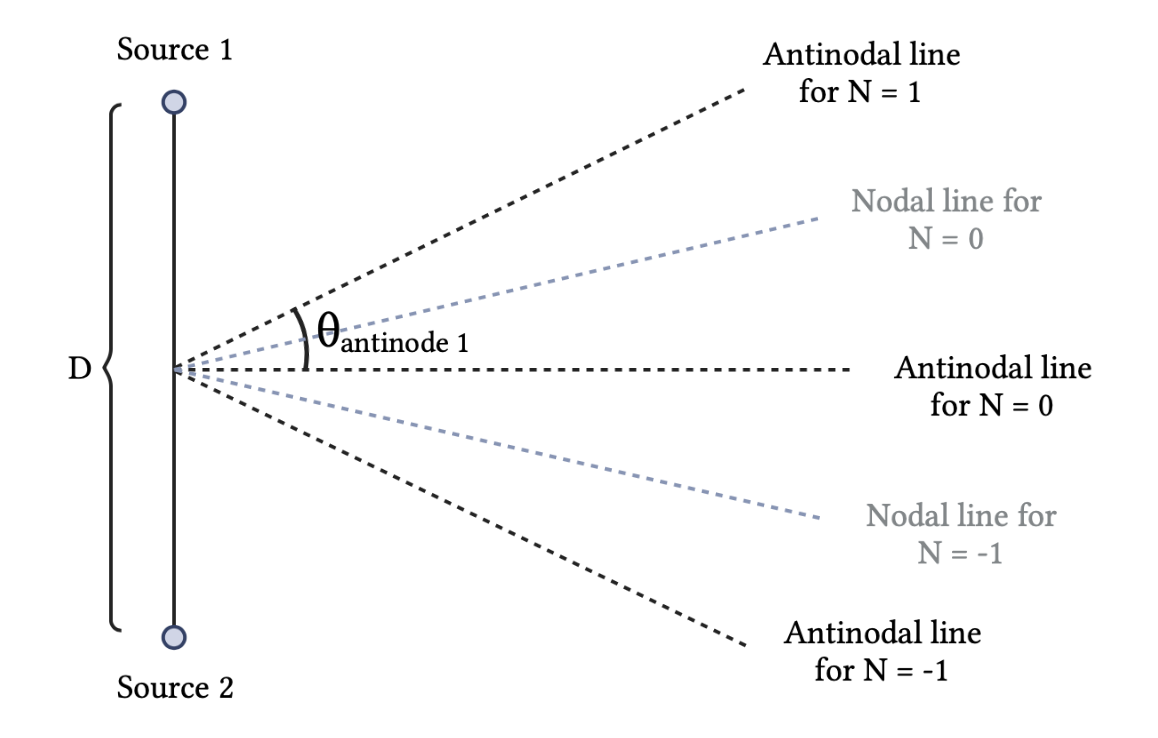
\includegraphics[height=7cm]{nodeantinodediagram}
			\caption{Antinodal and nodal lines diagram for the interference pattern generated by two circular wave sources}
		\end{figure}
		
		Diffraction occurs when a wave is partially blocked by objects. Considering a wavefront going through a small aperture, the direction in which its edges propagate is modified. This effect becomes more notorious as $\lambda$ approaches $d$, the latter being the width of the aperture. \\
		
		When using two slits, it can be seen how the initial plane waves show a similar pattern as that of the interference of two circular waves generated by point sources. %Huygens principle.
	\section{2 Material and Experimental Method}
	\subsection{2.1 Material}
	The used material consists in the following items:
	\begin{itemize}
		\item Tank with a water-detergent disolution
		\item Stroboscopic lamp
		\item Function generator with oscillating arm
		\item Fresnel lens
		\item Sheets of paper
		\item Ruler
		\item Calibre
		\item Protractor
		\item Mohr balance
		\item Rectangular plate, point generators and diffraction barriers
	
	\end{itemize}
	
	\subsection{2.2 Experimental method}
	The setup for this experience is rather simple, mainly consisting of a shallow tank (filled with the water-detergent disolution) and the generator.\\
	
	The generator counts with an arm and a small engine that shall make it oscillate and perturbe the disolution. It is connected to the lamp, which counts with a disc that shall rotate with the same frequency at which the arm oscillates in order to produce the stroboscopic effect. Between the lamp and the tank lays the Fresnel lens. \\
	
	White pieces of paper may be placed below the tank in order to easen the distinction of the fringes created by the waves due to the stroboscopic effect of the lamp (valleys shall appear as dark fringes and crests as light ones).\\
	
	It is important to measure the depth of the tank, checking the liquid is evenly distributed on it, as well as the density of the disolution.
	\subsubsection{2.2.1 Propagation of waves in water}
	For this assignment two different wave shapes are to be studied: plane and circular waves. The former shall be generated with the help of the straight edge whereas the latter are to be created by the pointlike pieces. These should be attached to the extremum of the oscillating arm and made sure not to hit the bottom of the tank while oscillating (either by adjusting the height of the arm or regulating the oscillation amplitude). The generated wavelengths shall be indirectly measured with a ruler for higher precision (the length of $m$ waves is measured and the result is then divided by this $m$ factor). This process is performed for several frequencies. Propagation velocities can be later estimated with the expressions of section 1. \\
	
	\subsubsection{2.2.2 Interference patterns}
 	The interference pattern to be observed is that of two circular waves. This can be achieved by attaching two point sources to the end of the oscillating arm. Adjustments on the frequency may be needed in order to correctly see the pattern. The measurements can be performed by marking the nodal lines on the paper and then measuring the angles they make with the normal with the protractor.
 	
 	\subsubsection{2.2.3 Diffraction patterns}
 	The diffraction patterns may be obtained by placing walls that obstruct the propagation of the waves, at an appropriate distance of each other ($\lambda \approx d$, where $d$ is the distance between the walls). Diffraction patterns for both single and double-slit setups are to be studied. For this section plane waves should be used, rather than circular.
	\section{3 Experimental Results and Questions}
	This section gathers the lab-measured quantities and the pertinent estimated values. For further details about the followed presentation criteria or the computed uncertainties please refer to the correspondent sections in the appendix. \\
	
	The experience has been performed with a dissolution of the following characteristics:
	\begin{table}[hbt!]
		\centering
		\begin{tabular}{|c | c|}
			\hline 
			$\boldsymbol{\sigma}$ \textbf{ (N/m)} & $(5.68 \pm 0.01) \cdot 10^{-2}$ \\
			\hline
			$\boldsymbol{\rho}$ \textbf{ (kg/m\textsuperscript{3})} & $ 998.7 \pm 0.1 $ \\
			\hline
		\end{tabular}
		\caption{Disolution characteristics}
	\end{table}

	and considering the value of gravity in the surface of Madrid as a theoretical value of $g = 9.8$ m/s\textsuperscript{2}.\textsuperscript{[2]}. \\
	The measurements have been taken for frequencies between 40 and 65 Hz due to the limitations fo the stroboscopic system.
	\subsection{3.1 Propagation of waves in water}
	\subsubsection{3.1.1 Regime of propagation}
		The depth of the tank $h$ has been determined to be equal to 1.30 $\pm$ 0.01 cm. One can see in table TK the highest wavelengths are those measured at frequencies $f = 40$ Hz, ($\lambda_{plane} = TK$, $\lambda_{circular} = TK$) this being a reason why it can be said that the propagations occur in the deep regime. It is seen that $h \approx 2\lambda \geq 0.5\lambda$. \\
	\subsubsection{3.1.2 $\lambda$ of plane and circular waves}
		Table TK shows the measured values for the wavelength of the plane and circular waves at different frequencies.
		
		\begin{table}[hbt!]
			\centering
			\begin{tabular}{|c|c|c|}
				\hline
					$\boldsymbol{f} $ \textbf{(Hz)} & $ \boldsymbol{\lambda_{p}} $ \textbf{(mm)} & $ \boldsymbol{\lambda_{c}} $ \textbf{(mm)} \\
				\hline
				\hline
				$40 \pm 1$ & $5.6 \pm 0.1$ & $5.7 \pm 0.1$ \\
				
				$45 \pm 1$ & $5.2 \pm 0.1$ & $5.2 \pm 0.1$\\
			
				$50 \pm 1$ & $4.9 \pm 0.1$ & $4.8 \pm 0.1$\\
				
				$55 \pm 1$ & $4.5 \pm 0.1$ & $4.4 \pm 0.1$\\
				
				$60 \pm 1$ & $4.2 \pm 0.1$ & $4.2 \pm 0.1$\\
			
				$65 \pm 1$ & $3.9 \pm 0.1$ & $3.8 \pm 0.1$\\
				\hline
				
			\end{tabular}
			\caption{Wavelengths of the plane ($\lambda_p$) and circular ($\lambda_c$) waves in terms of the frequency}
		\end{table}
		It can be seen that the values for the wavelength for both the plane and circular waves are compatible with each other in all frequencies. This is expected since the wavelength of any wave (either electromagnetic or mechanic) should not depend on the wave geometry. %This can be explained through equations 1 and 3. Equation 1 establishes a relation between $\lambda$, $f$ and the propagation speed, and it can be seen in equation 3 that for non dispersive homogeneous media, the propagation speed of mechanical waves can be entirely determined by properties of these media.
%	\subsubsection{3.1.3 Observations}
	\subsubsection{3.1.3 Phase velocity in terms of $\lambda$}
		Since the values of $\lambda_p$ and $\lambda_c$ are very close to and compatible with each other at all frequencies, from equation 1 it can be seen that so shall be the phase velocities for the frequencies. Therefore, only the $\lambda_p$ results may be considered for this section. Table 3 displays a comparison of the obtained velocities for each wavelength by using equation 1 and the approximation of the deep water regime (eq. 4). \\
		
		\begin{table}[hbt!]
			\centering
			\begin{tabular}{|c|c|c|}
				\hline
					\textbf{$\boldsymbol{\lambda_p}$ (mm)} & \textbf{$\boldsymbol{v_p}$ (1) (m/s)} & \textbf{$\boldsymbol{v_p} $ (4) (m/s)} \\
					\hline
					\hline
					5.6 $\pm$ 0.1 & 0.2240 $\pm$ 0.0069 & 0.2693 $\pm$ 0.0018 \\
					5.2 $\pm$ 0.1 & 0.2340 $\pm$ 0.0069 & 0.2772 $\pm$ 0.0021 \\
					4.9 $\pm$ 0.1 & 0.2450 $\pm$ 0.0070 & 0.2839 $\pm$ 0.0024 \\
					4.5 $\pm$ 0.1 & 0.2475 $\pm$ 0.0071 & 0.2940 $\pm$ 0.0027 \\
					4.2 $\pm$ 0.1 & 0.2520 $\pm$ 0.0073 & 0.3027 $\pm$ 0.0031 \\
					3.9 $\pm$ 0.1 & 0.2535 $\pm$ 0.0076 & 0.3126 $\pm$ 0.0035 \\
				\hline
			\end{tabular}
		\caption{Real $v_p$ vs deep regime approximation for each $\lambda$}
		\end{table}
		These values can be presented in a graph.
		
		\begin{figure}[hbt!]
			\centering
			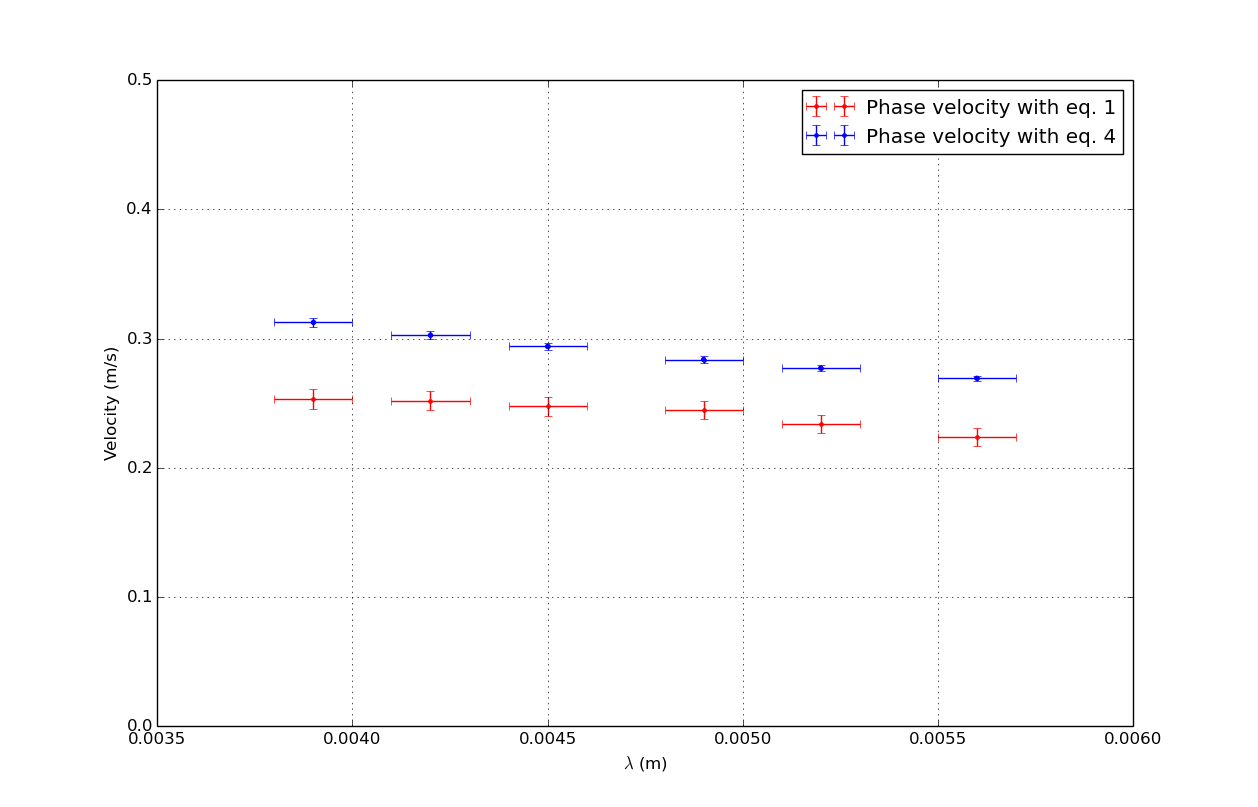
\includegraphics[height=6cm]{approx}
			\caption{Comparison among propagation speeds yielded by each equation}
		\end{figure}
		
		It is clearly seen the values provided by the eq. 4 (which shall be referred to as the approximation from now on) are higher by a factor of about 5 cm/s. Apart from this, the results follow a similar behaviour, the speed slightly decreasing as the $\lambda$ increase.\\

	
		Bear in mind the shallow regime approximation implies the disolution does not conform a dispersive medium, this meaning it yields the same speed value for any wavelength: $v_{p_{shallow}} = 0.3569 \pm 0.0014$ m/s. It can be seen this value lays farther from the values of equation 1 than any found with the deep regime approximation, another reason that supports this motion occurs under the conditions fulfiling the latter regime. As a consequence, it is not too bold to state equation 4 is more appropriate in this case.
	

		
		\subsubsection{3.1.4  Dispersion relation $\omega(\kappa)$ and group velocity}
		The dispersion relation $\omega(\kappa)$ may be easily derived from the deep water approximation (eq. 4) and the relation of $v, f$ and $\lambda$ (eq. 1). \\
		
			From equations (1) and $\omega = 2\pi f$:
			\begin{align*}
				f = \frac{v}{\lambda} &\implies \omega = \frac{2\pi}{\lambda} v = \kappa v 
				\mbox{, and }\\
				v \approx \sqrt{\frac{g\lambda}{2\pi} + \frac{2\pi \sigma}{\rho \lambda}} &=   \sqrt{\frac{g}{\kappa} + \frac{\kappa \sigma}{\rho}}
			\end{align*}\\
		
		Therefore,
			\begin{equation}\label{wk}
				\omega(\kappa) = \kappa \sqrt{\frac{g}{\kappa} + \frac{\kappa \sigma}{\rho}}
			\end{equation}\\
		
		The group velocity $v_g$ can be computed as the derivative of the dispersion relation i.e. expression \ref{wk}.
		
		\begin{equation}\label{vg}
		v_g = \frac{d\omega}{d\kappa} = \frac{g\rho + 3\kappa^2\sigma}{2\kappa\rho \sqrt{\frac{g}{\kappa} + \frac{\kappa \sigma}{\rho}}}
		\end{equation}
		
		\subsubsection{3.1.5 Group and phase velocities}
		Figure 3 displays the curves of the phase and group velocities of the wave in terms of its wavelength.
		
		\begin{figure}[h!]
			\centering
			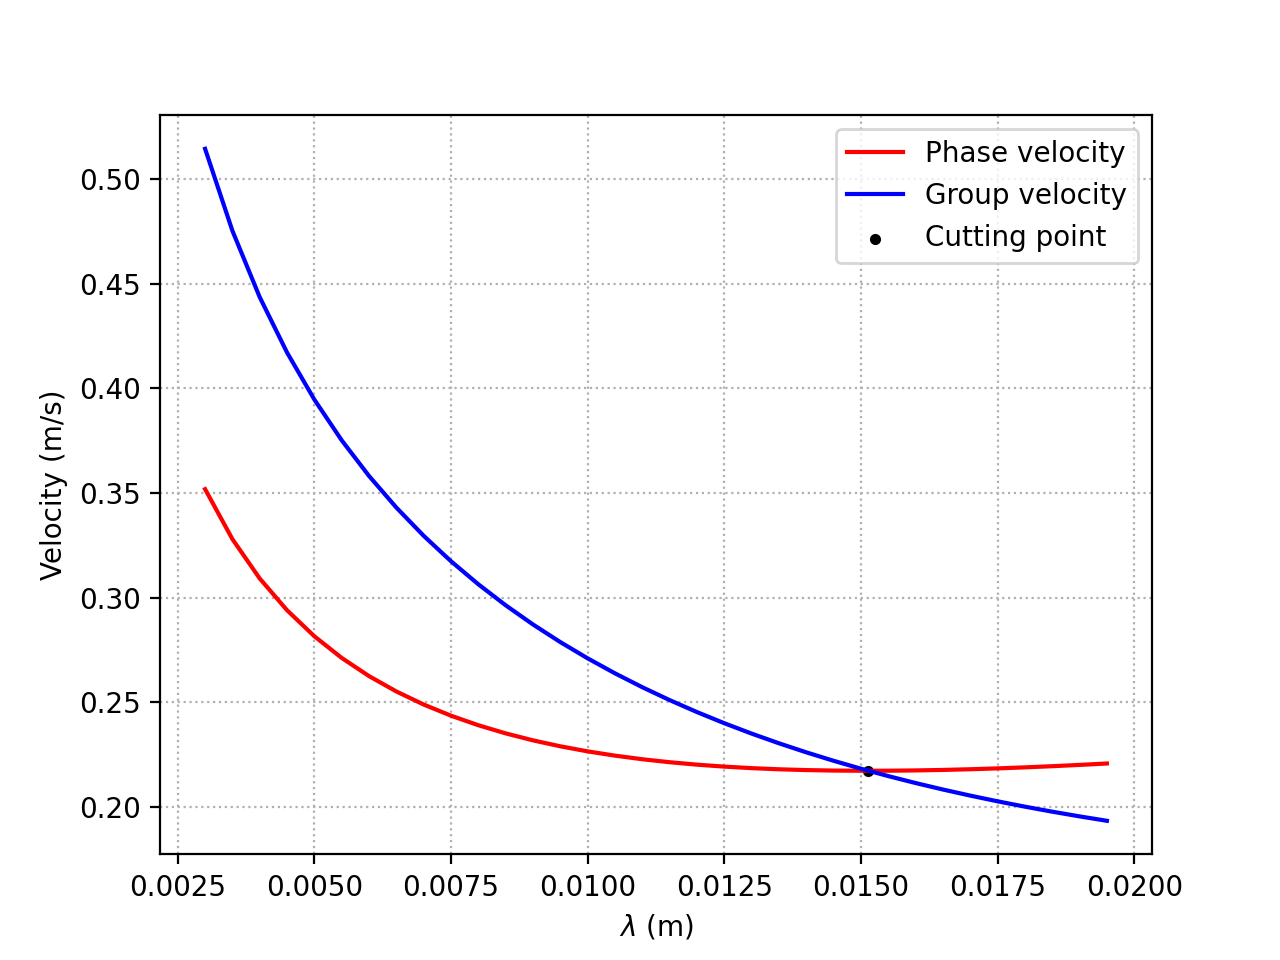
\includegraphics[height=7cm]{cutvelocity}
			\caption{Group and phase velocities in terms of $\lambda$}
		\end{figure}
	In order to compute the point at which both curves intersect, one may try to make equations \ref{vpdeep} and \ref{vg} equal.

	\begin{align} 
		v = v_g &\implies \sqrt{\frac{g}{\kappa} + \frac{\kappa \sigma}{\rho}} = \frac{g\rho + 3\kappa^2\sigma}{2\kappa\rho \sqrt{\frac{g}{\kappa} + \frac{\kappa \sigma}{\rho}}}; \nonumber\\
		2\kappa \rho \left(\frac{g}{\kappa} + \frac{\kappa \sigma}{\rho}\right) = g\rho + 3\kappa^2\sigma &\implies 2g\rho + 2\kappa^2\sigma = g\rho + 3\kappa^2 \sigma; \nonumber \\
		 \frac{g\rho}{\sigma} = \kappa^2 &\implies \lambda_{eq} = 2\pi \sqrt{\frac{\sigma}{g\rho}}
	\end{align}

	Substituting the values, it shall be found that the group and phase velocities are equal for $\lambda_{eq} = 0.015136 \pm 0.000013 $ m. It can be quickly checked that \begin{align*}\label{speedcheck}
		v (\lambda_{eq}) &= \sqrt{\frac{g\lambda_{eq}}{2\pi} + \frac{2\pi\sigma}{\rho\lambda_{eq}}} = 0.2173 \mbox{ m/s}\\ 
		v_g (\lambda_{eq}) &= \frac{g\rho + 12\left(\frac{\pi}{\lambda_{eq}}\right)^2\sigma}{\frac{4\pi}{\lambda_{eq}}\rho \sqrt{\frac{g\lambda_{eq}}{2\pi} + \frac{2\pi \sigma}{\rho\lambda_{eq}}}} = 0.2174 \mbox{ m/s}
	\end{align*} 
	which are the results one would expect after seeing the previous graph (i.e. figure 3).
	\subsection{3.2 Interference of surface waves}
	The interference patterns have been studied with two point sources separated at a distance $D$ from each other. Figure 4 shows the observed pattern.\\
	\begin{figure}[h!]
		\centering
		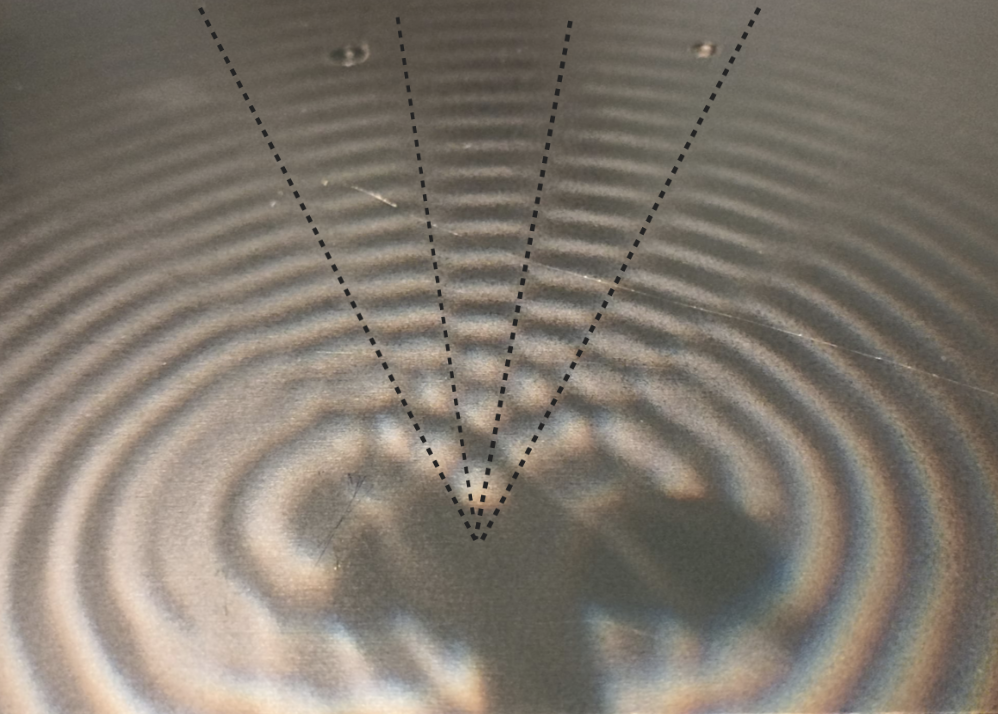
\includegraphics[height=7cm]{ipat}
		\caption{Interference of two circular waves. The nodal lines are marked with dotted lines}
	\end{figure}

	It can be seen there are points at wich the interference of the waves is fully destructive. These points form what may be called nodal lines, they being straight lines that origin at the middle point between both sources and extend at different angles $\theta_N$ from the normal to the line that joins both sources (Figure 1). From the nodal lines equation, it can be fast found that \begin{equation}\label{thetan}
		\theta_N = \arcsin\left(\frac{2N + 1}{2 D} \lambda \right), \mbox{ } N \in \mathbb{Z}.
	\end{equation}
	Assuming $\frac{2N + 1}{2D}\lambda \leq 1$, it can be seen amplitudes are inversely proportional to the distance $D$ between the sources and directly proportional to the wavelengths. Since propagation speed does not vary greatly with the wavelength (as checked in section 3.1), it can be stated that the amplitudes should also decrease with the frequency. \\
	
	Measuring the nodal lines for a frequency of 38 Hz ($\lambda = 5.9 \pm 0.1 $ mm), the found angles for the first nodal lines have been are the following:
	\begin{table}[hbt!]
		\centering
		\begin{tabular}{|c|c|}
			\hline
			$\boldsymbol{N}$ & $\boldsymbol{\theta_N}$ \textbf{(rad)} \\
			\hline
			-3 & -0.681 $\pm$ 0.017 \\
			-2 & -0.393 $\pm$ 0.017 \\
			-1 & -0.131 $\pm$ 0.017 \\
			0 & 0.148 $\pm$ 0.017 \\
			1 & 0.445 $\pm$ 0.017 \\
			2 & 0.742 $\pm$ 0.017 \\
			\hline
		\end{tabular}
		\caption{Experimental angles for $D = 2$ cm and $f = 38$ Hz}
	\end{table}
	
	These are not exactly symmetric, what might have been due to a misplacement of the centre of the protractor. The previous values can be compared to the theoretical ones, the latter resulting from equation \ref{thetan}.
	\begin{table}[hbt!]
		\centering
		\begin{tabular}{|c|c|}
			\hline
			$\boldsymbol{N}$ & $\boldsymbol{\theta_N}$ \textbf{(rad)} \\
			\hline
			-3 & -0.738 $\pm$ 0.048 \\
			-2 & -0.443 $\pm$ 0.025 \\
			-1 & -0.1475 $\pm$ 0.0078 \\
			0 & 0.1475 $\pm$ 0.0078 \\
			1 & 0.443 $\pm$ 0.017 \\
			2 & 0.738 $\pm$ 0.048 \\
			\hline
		\end{tabular}
		\caption{Theoretical angles for $D = 2$ cm and $f = 38$ Hz}
	\end{table}

	The experimental angles for the negative $N$ are smaller than they should while the non-negative $N$ display slightly experimental values, what follows again from the protractor misplacement when measuring. \\
	
	It can now be checked that the $\theta_N$ decrease as the values of $D$ and $f$ get vary as expected:
	
	\begin{itemize}
		
		\item [i)] Increasing the frequency to f = 48 Hz:
		
\begin{table}[hbt!]
	\centering
	\begin{tabular}{|c|c|c|}
		\hline
		$\boldsymbol{N}$ & $\boldsymbol{\theta_N}$ \textbf{theor. (rad)} & $\boldsymbol{\theta_N}$ \textbf{exp. (rad) } \\
		\hline
		-2 & -0.375 $\pm$ 0.021 & -0.358 $\pm$ 0.017 \\
		-1 & -0.1250 $\pm$ 0.0068& -0.113 $\pm$ 0.017 \\
		0 & 0.1250 $\pm$ 0.0068 & 0.122 $\pm$ 0.017\\
		1 & 0.375 $\pm$ 0.017&  0.367 $\pm$ 0.017\\
		\hline
	\end{tabular}
	\caption{Experimental angles for $D = 2$ cm and $f = 48$ Hz}
\end{table}

\item [ii)] Decreasing the distance between sources to $D = 1.5$ cm


	\begin{table}[H]
		\centering
		\begin{tabular}{|c|c|c|}
			\hline
			$\boldsymbol{N}$ & $\boldsymbol{\theta_N}$ \textbf{theor. (rad)} & $\boldsymbol{\theta_N}$ \textbf{exp. (rad) } \\
			\hline
			-2 & -0.590 $\pm$ 0.046 & -0.576 $\pm$ 0.017 \\
			-1 & -0.197 $\pm$ 0.014& -0.192 $\pm$ 0.017 \\
			0 & 0.197 $\pm$ 0.014 & 0.209 $\pm$ 0.017\\
			1 & 0.590 $\pm$ 0.046&  0.628 $\pm$ 0.017\\
			\hline
		\end{tabular}
		\caption{Experimental angles for $D = 1.5$ cm and $f = 38$ Hz}
	\end{table}
\end{itemize}

It can be seen that most of the results are compatible, and behave as expected (decreasing as $f$ was increased and increasing when $D$ was made smaller).
	\subsection{3.3 Diffraction of surface waves}	
	\subsubsection{3.3.1 One-slit diffraction pattern}
	When studying the diffraction pattern generated by one unique slit and plane waves two parallelepipeds have been placed in the liquid (at some distance from the plane edge generating the waves), making sure the distance $d$ among these is similar to the wavelength.\\\
	\begin{figure}[hbt!]
		\centering
		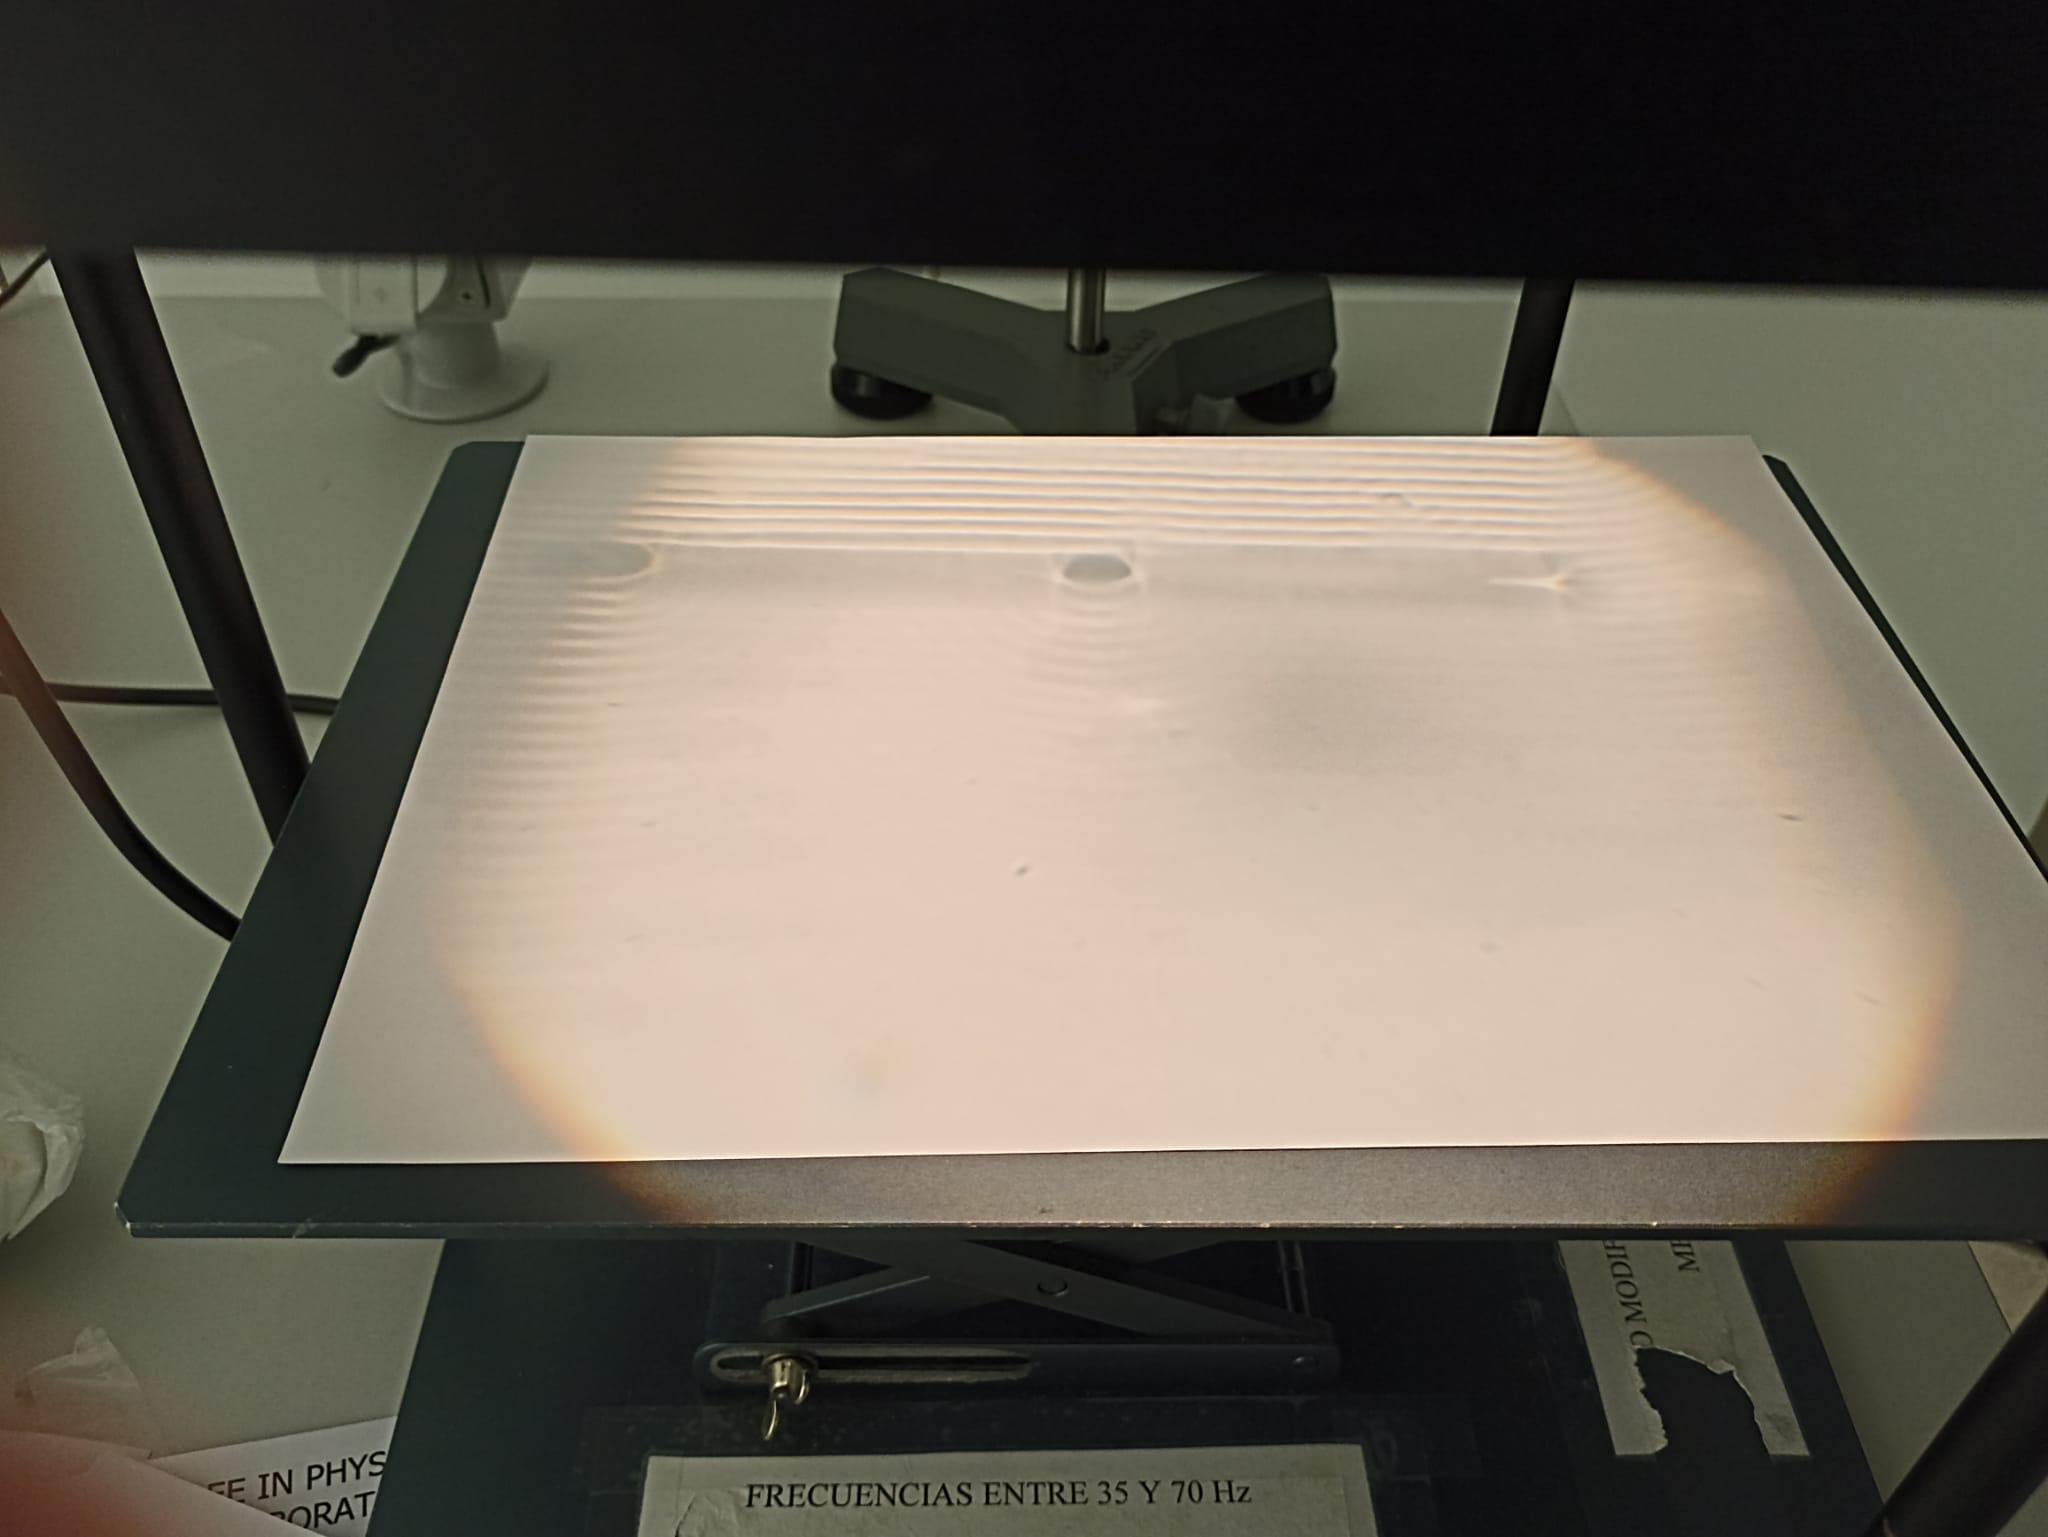
\includegraphics[height=9.5cm]{1slit}
		\caption{Strong diffraction pattern of plane waves going through one slit}
	\end{figure}

	Figure 5 shows the diffraction pattern of a single slit. It can be appreciated that the plane wavesfronts curve and behave as those origined by a point source. The frequency of the waves remains constant during the process, and so their phase speed and wavelength, for none of these quantities depend on the geometry of the wavefronts. \\
	
	Figure 6 shows that, when the distance between walls is increased and made much higher than the wavelength diffraction is weaker and so waves remain plane.
	\begin{figure}[hbt!]
		\centering
		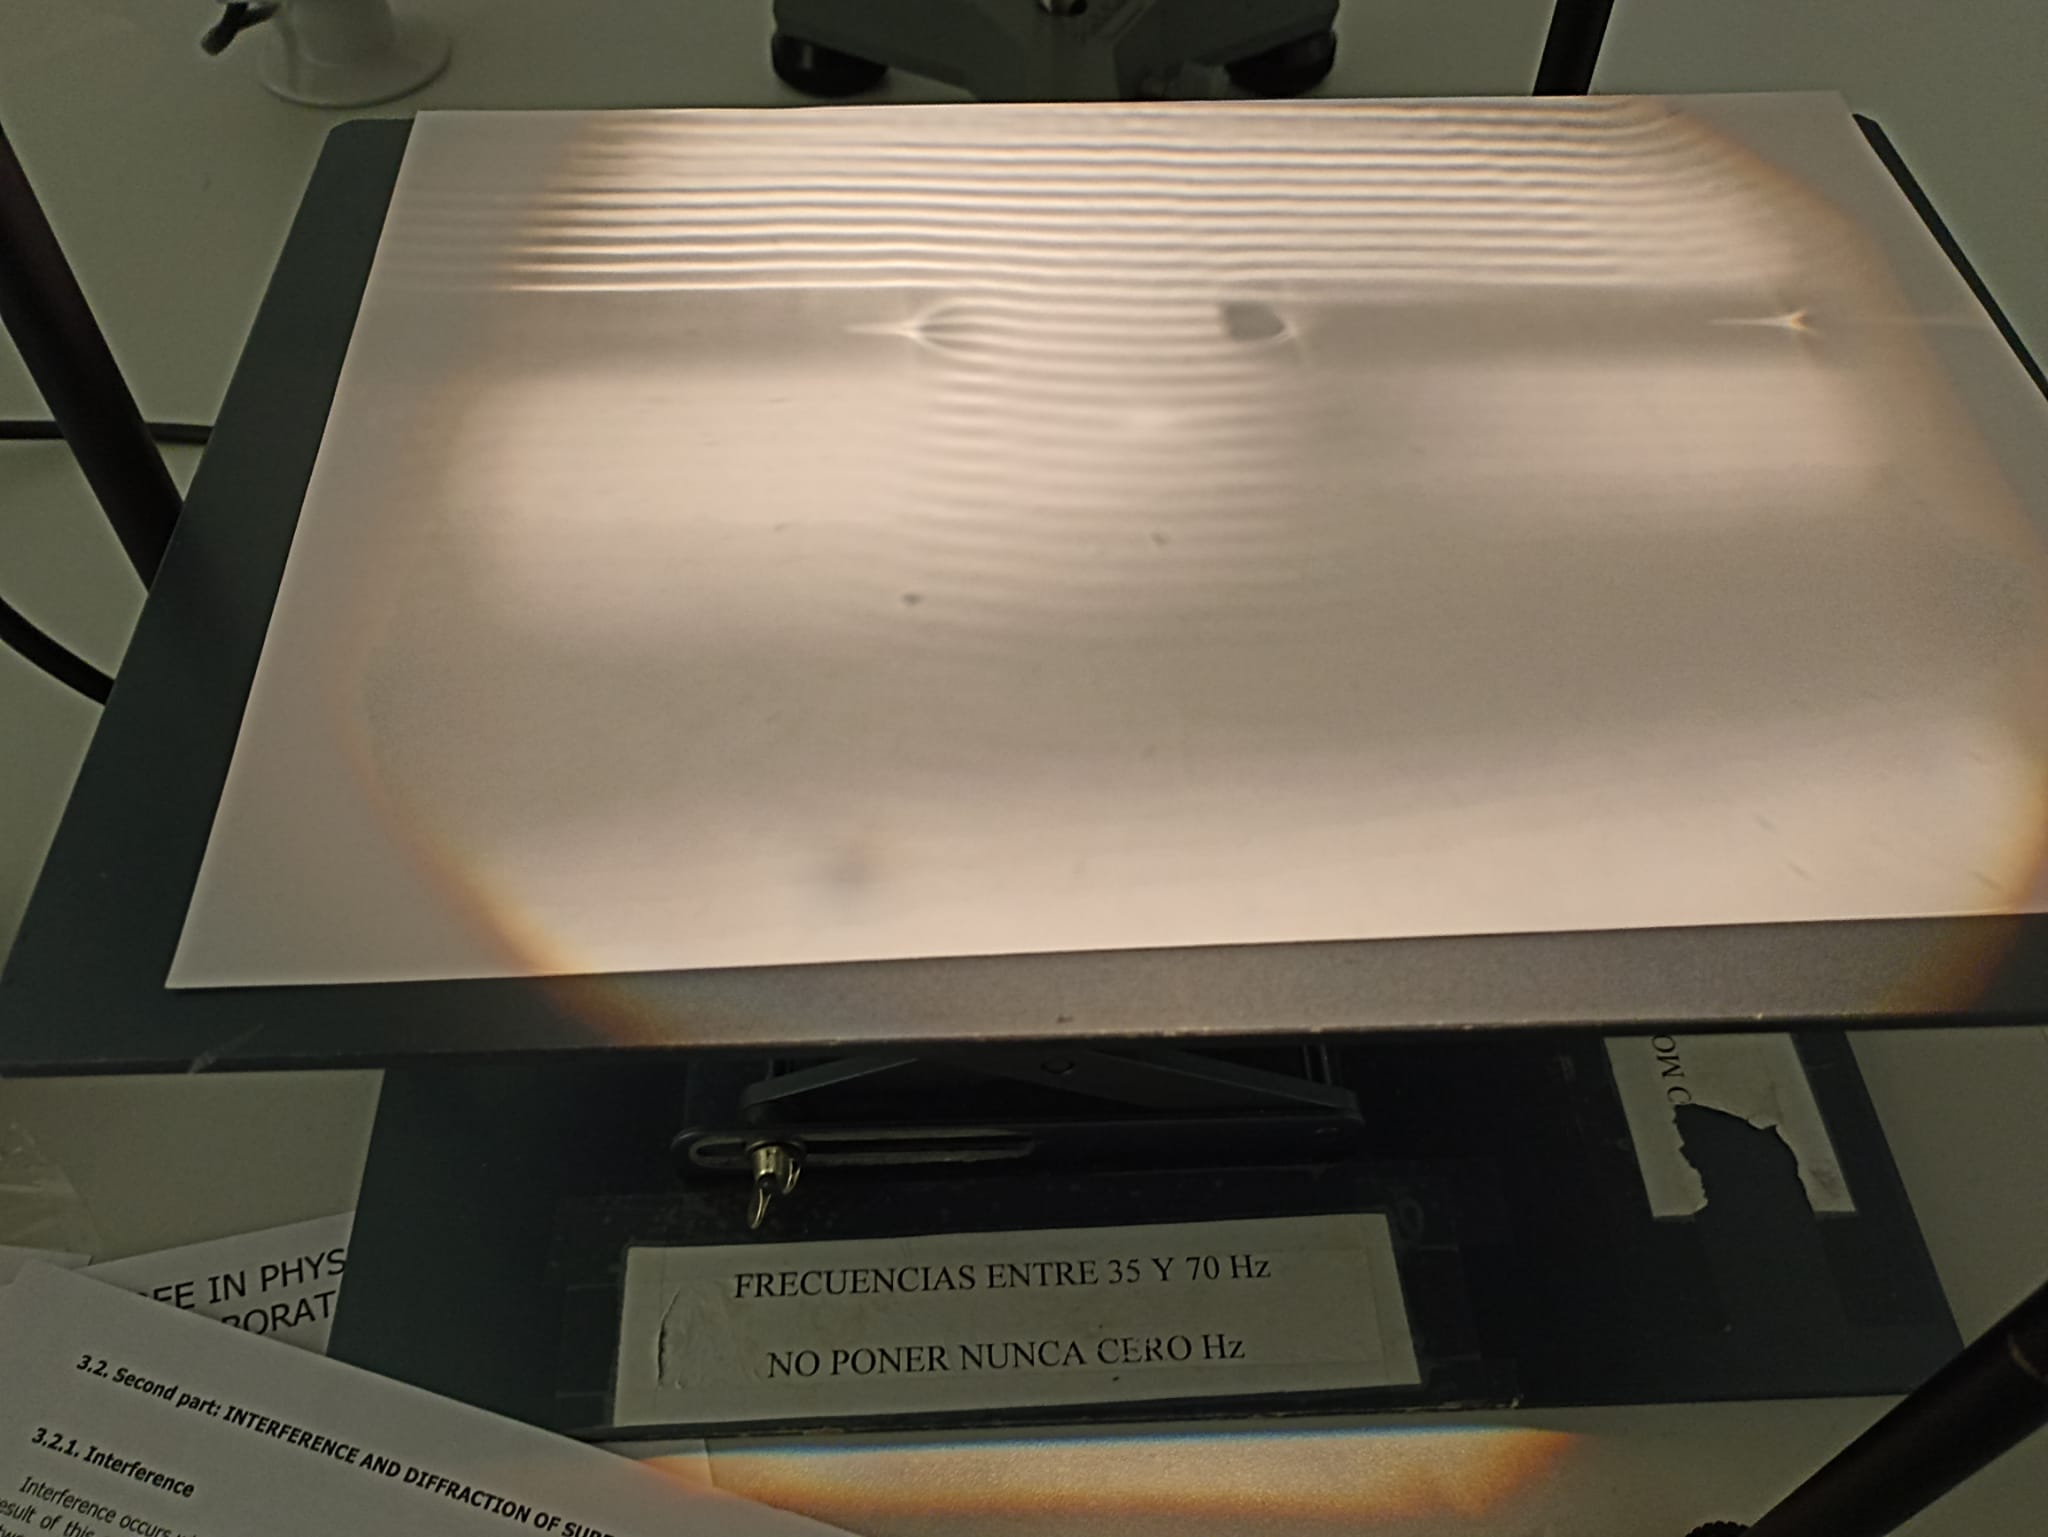
\includegraphics[height=9.5cm]{1slitw}
		\caption{Weak diffraction pattern of plane waves going through one slit}
	\end{figure}
	\newpage
	\subsubsection{3.3.2 Double-slit diffraction pattern}
	When dealing with double slits, diffraction is similar to that with one slit (the holes behave as sources of circular waves), with the major difference that now there is interference between the new circular waves, which generate similar maxima and minima to those observed in Young's experiment.
	\begin{figure}[hbt!]
		\centering
		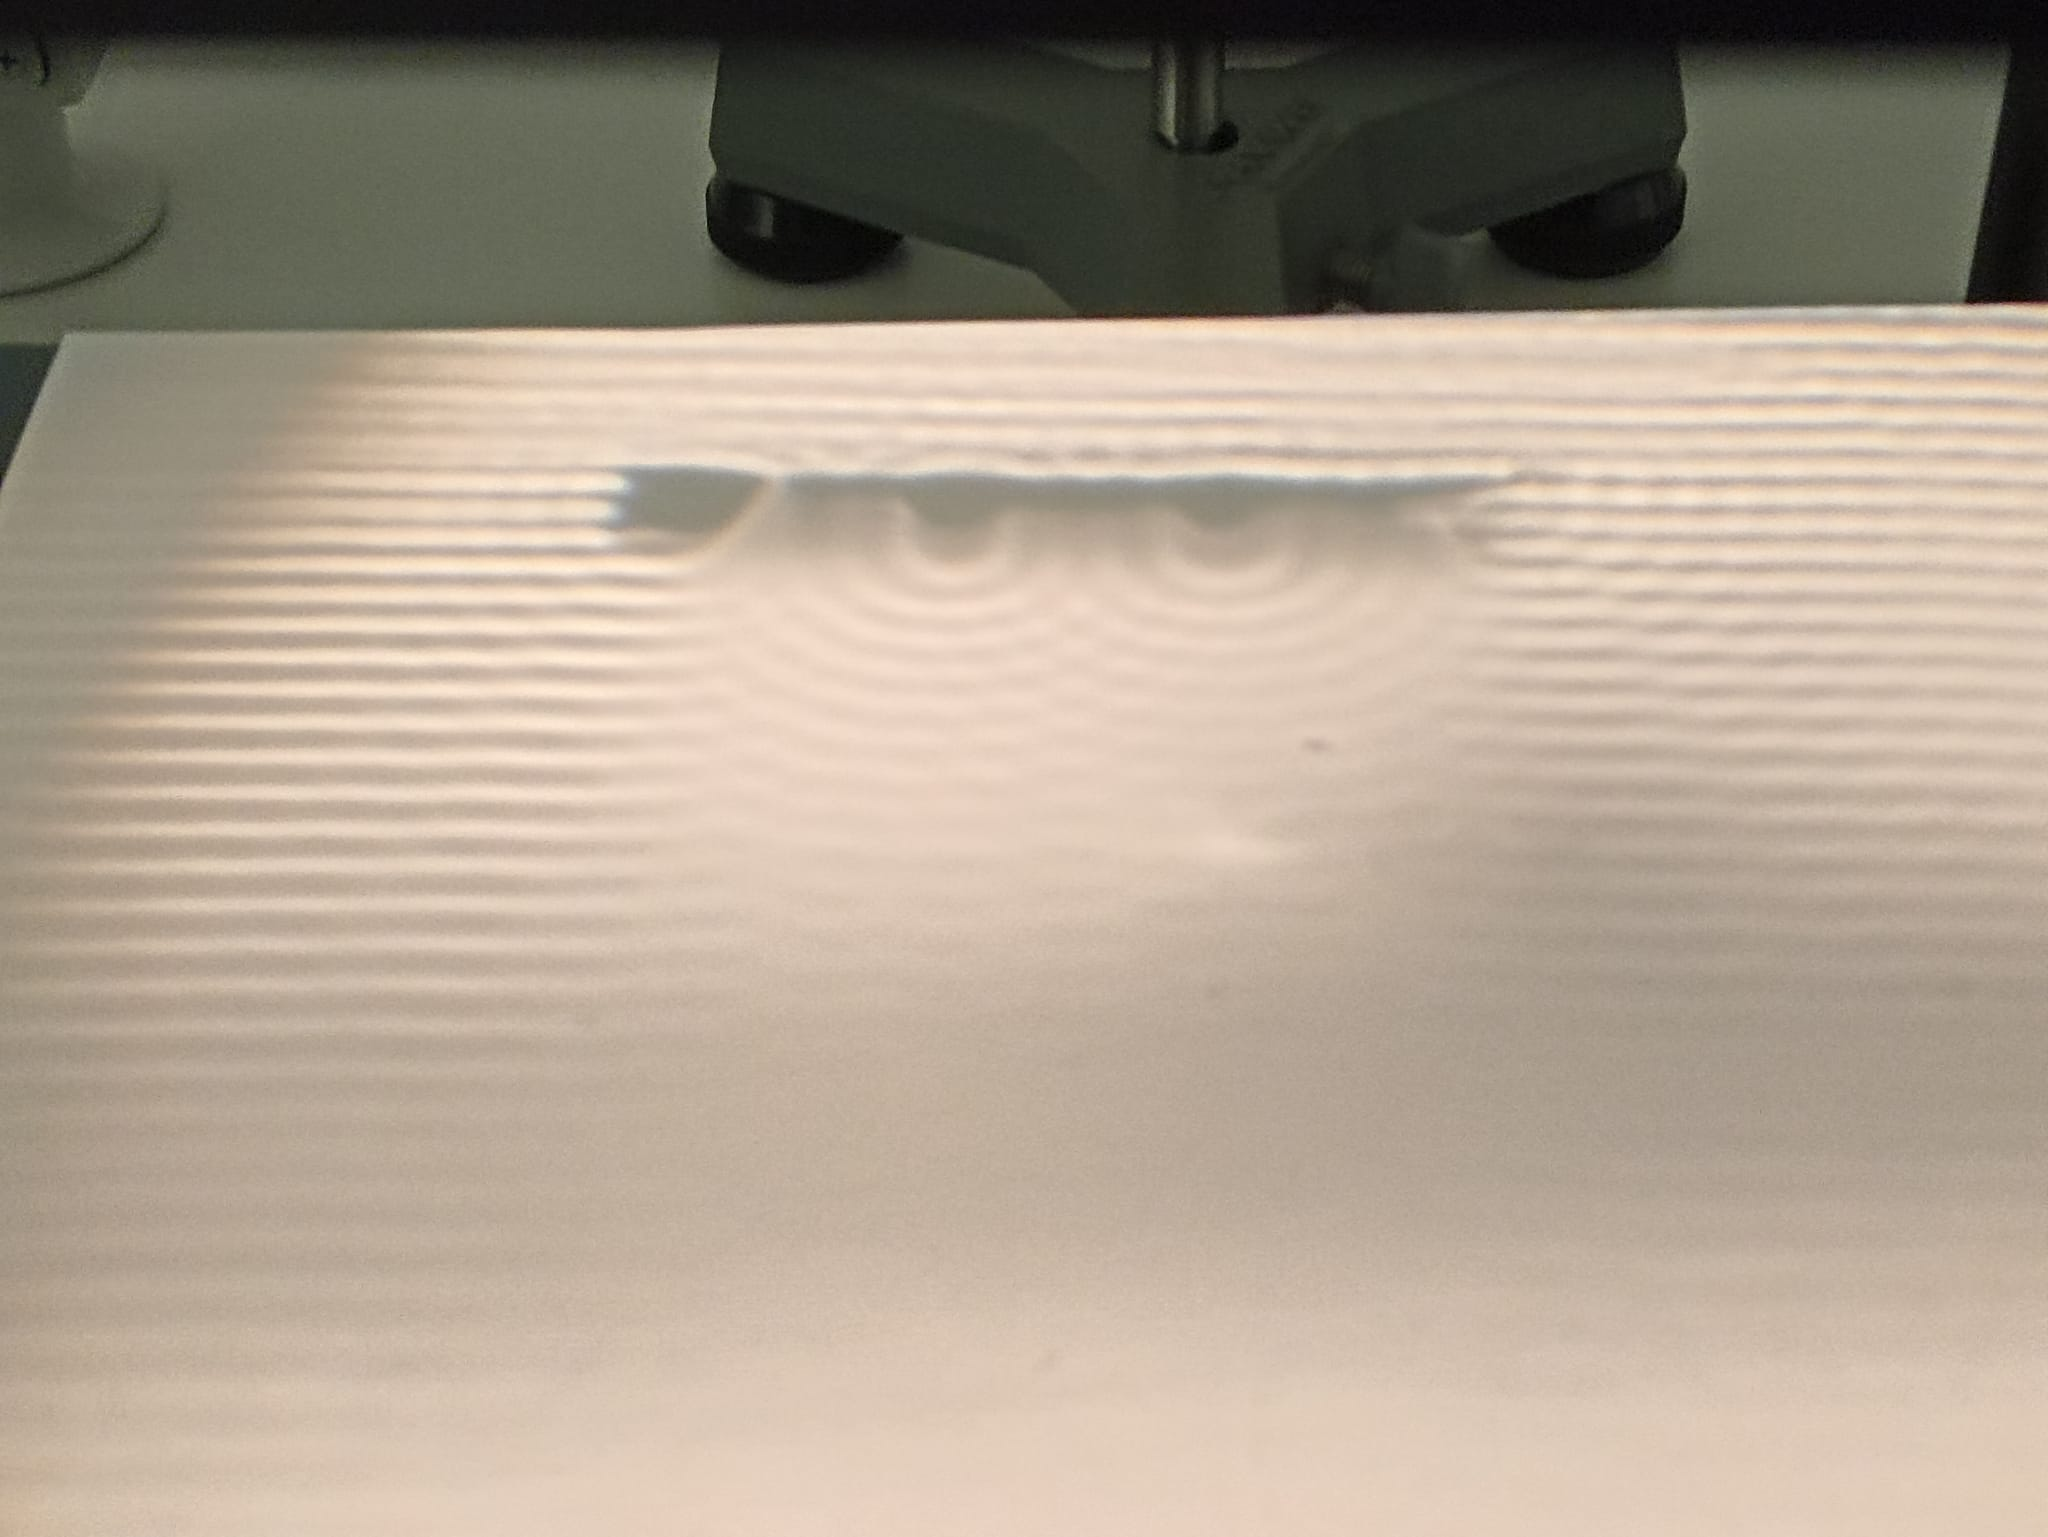
\includegraphics[height=9.5cm]{2slit}
		\caption{Diffraction pattern of plane waves going through a double-slit system}
	\end{figure}
	\section{4 Conclusion}
	The results of this experience are quite satisfactory. They are coherent, accurate (being many of the experimental values compatible with those which were theoretically estimated) and precise, the highest relative uncertainties of about 8\%. The velocity approximations in the deep regime show a notoriously high but almost constant deviation, between $20$ and $23 \%$.\\
	
The main difficulty of the practical was taking the measurements, this task being hard due to imprecissions when sketching the guiding lines to later evaluate the measured quantities. This includes drawing the normal that crosses the middle point of the line joining the two sources when measureng the nodal lines of the interference patterns.
	\section{References}
	[1] ``Laboratory of Mechanics and Waves: Ripple Tank" Complutense University of Madrid, 2021.\\
	
	[2] Rodríguez Pujol, E. (2005). ``\textit{Absolute Gravity Network in Spain}" %(Vol. 17, pp. 147–163). Madrid, Spain: Ediciones Complutense. 
	
	\newpage
	
	\section{Appendix}

	\subsection{A.1 Presentation of results}
	Experimental results have been rounded considering up to two significant figures in their uncertainties. Tabular of theoretical values have been presented without uncertainties, rounded to the same decimal figures as their corresponding experimental results unless they being exact.\\
	
	The priorities when displaying data has been making it easy to read, this being the reason why not necessarily all quantities are presented in units of the International System of Units. For instance, many distance measurements are shown in milimetres (mm). \\
	\subsection{A.2 Error estimation}
	\subsubsection{A.2.1 Direct measurements}
	Direct measurements present errors that depend directly on the precision of the used measuring devices. For instance, angles are presented with an uncertainty of 1º (0.017 rad), this being the precision of the protractor, and distances present 1 mm of uncertainty. \\
	
	 Wavelengths, however, present a tenth of this, since 10 wavelengths were measured and it was considered that $\Delta (10\lambda) = 10 \Delta \lambda$.
	\subsubsection{A.2.2 Indirect measurements}
	The following equations have been employed in the calculation of the uncertainties of other measurements:
	\begin{equation}\label{deltalambda}
		\Delta \lambda = \frac{1}{10} \Delta (10\lambda)
	\end{equation}
	\begin{equation}\label{deltavp1}
		\Delta v_{p_1} = \sqrt{(f\Delta \lambda) + (\lambda \Delta f)^2}
	\end{equation}
	\begin{equation}\label{deltavp4}
		\Delta v_{p_4} = \frac{\pi}{v_{p_4}\rho\lambda}\sqrt{\left[\left(\frac{g\rho\lambda}{4\pi^2} - \frac{\sigma}{\lambda}\right)\Delta\lambda\right]^2 + \Delta \sigma^2 + \left(\frac{\sigma\Delta\rho}{\rho}\right)^2}
	\end{equation}
	\begin{equation}\label{deltatheta}
		\Delta \theta = \left|\frac{\Delta \sin \theta}{\sqrt{1-\sin^2\theta}}\right| = |\tan \theta|\sqrt{\left(\frac{\Delta \lambda}{\lambda}\right)^2 + \left(\frac{\Delta D}{D}\right)^2}
	\end{equation}
	\subsubsection{A.2.3 Other error computations and deviations}
	\begin{itemize}
		\item Deviation from theoretical values:
		\begin{equation}\label{dev}
			\delta (\%) = 100 \cdot \frac{|X_{exp} - X_{theor}|}{X_{theor}}
		\end{equation}
		\item Relative uncertainty:
		\begin{equation}\label{drel}
			\delta_{rel} (\%) = 100 \cdot \frac{\Delta X}{X}
		\end{equation}
		
	\end{itemize}
\end{document}